\chapter*{Annexe du chapitre \ref{chap:methodes}: Structures de données dans proteus}
\label{chap:annexeproteus}

Cette annexe présente les principales structures de données utilisées dans le programme proteus. Un premier ensemble de structures regroupe les données physiques fournies en entrée à proteus, voir la figure \ref{fig:structPhy}. Le fichier backbone contient, d'une part, la description de tous les rotamères possibles à chaque position du système et d'autre part les énergies propres de chacun de ces rotamères. La structure \verb!residues! contient la totalité de ces rotamères. Ils sont regroupés dans un tableau \verb!rotamers!  pour chaque type. L'ensemble des types est regroupé à son tour dans un tableau \verb!types!. La matrice \verb!ener! regroupe les énergies de paires dans un tableau à deux dimensions représentant les couples de positions $(i,j)$. Chaque élément de ce tableau contient l'ensemble des couples de rotamères de $(i,j)$  sous forme de tableau à deux dimensions.
   \begin{figure}[!htbp]
     \centering
     \begin{tabular}{c}
       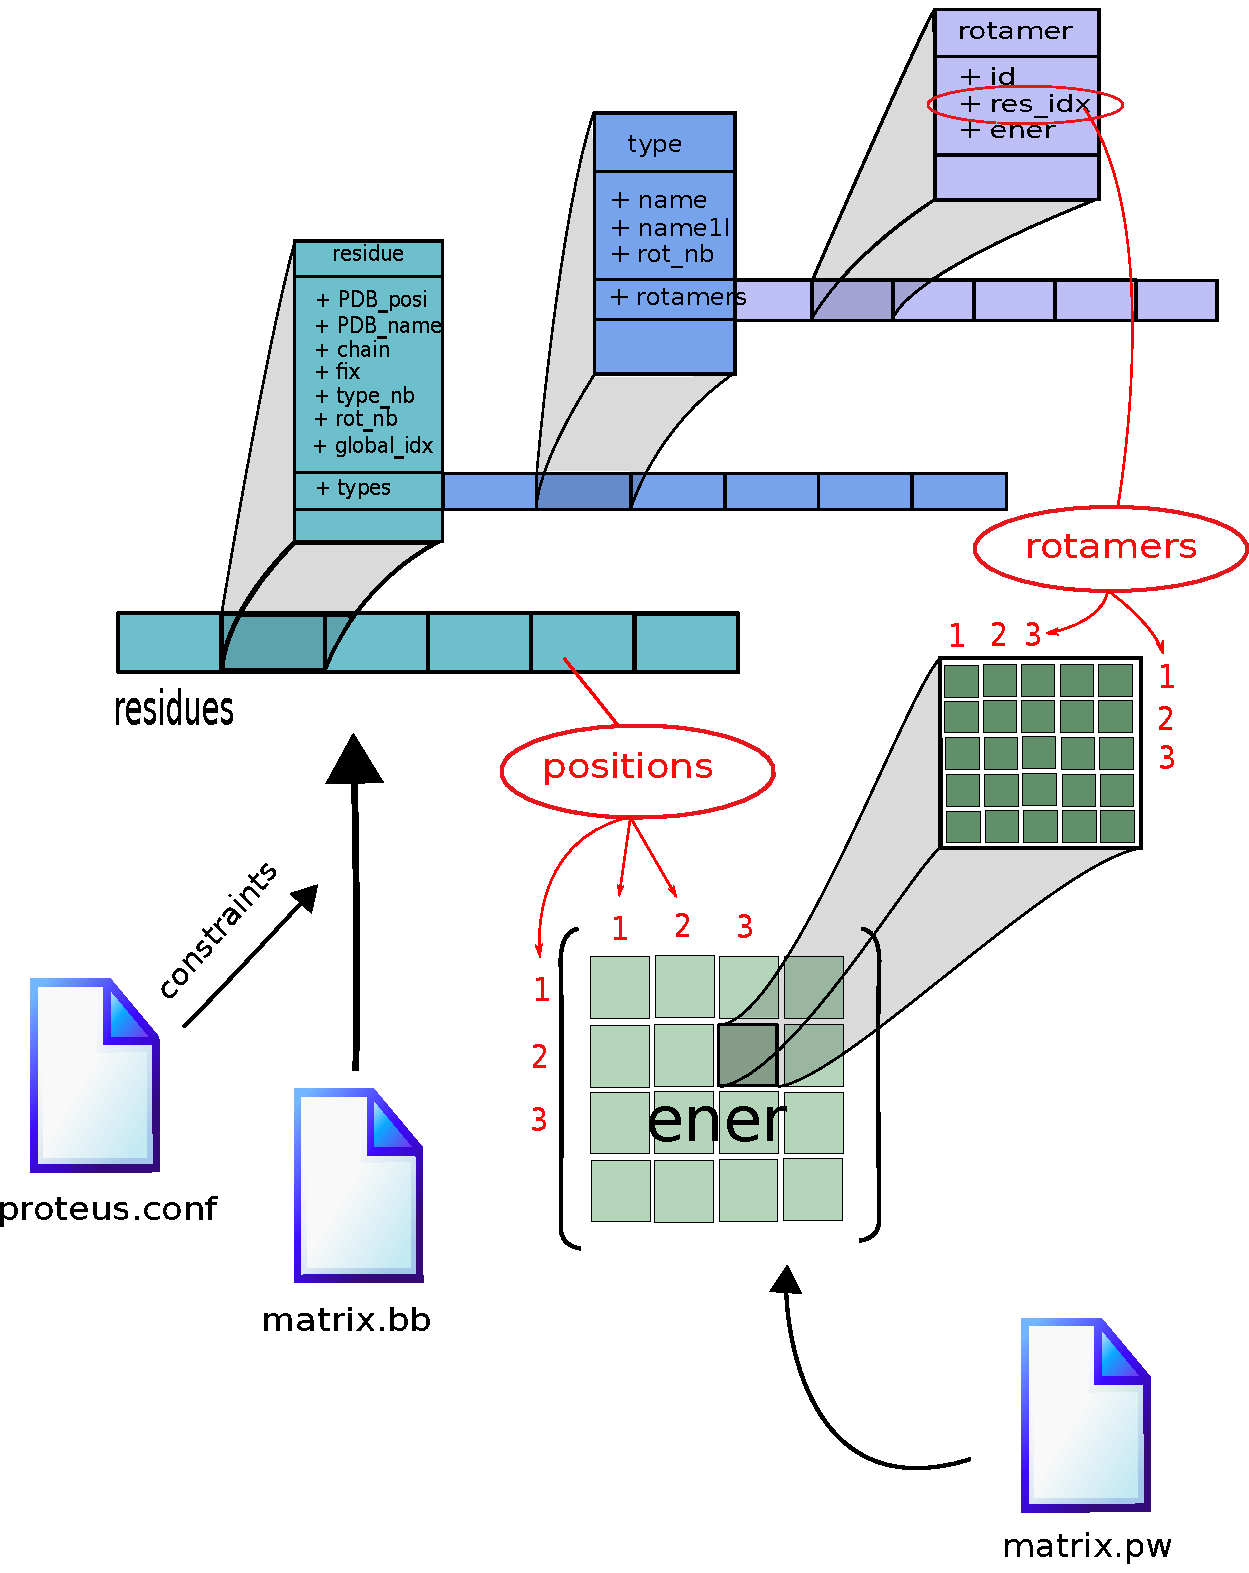
\includegraphics[width=13cm]{figure/structures_physique.pdf} 
     \end{tabular}
     
     \caption{Les principales structures \og physiques\fg  dans proteus}
\label{fig:structPhy}
   \end{figure}

Le deuxième ensemble est constitué des structures \og logiques \fg. Ce sont elles qui gèrent la duplication de parties du système comme expliqué à la section \ref{sub:group}. La structure \verb!posi_instance! contient un ensemble d'index sur un ensemble d'éléments des tableaux \verb!rotamers! permettant la définition d'un espace d'état qui lui est propre. La structure \verb!group! contient une liste de \verb!posi_instance!. Cela est détaillé à la figure  \ref{fig:structLog}.    
   \begin{figure}[!htbp]
     \centering
     \begin{tabular}{c}
       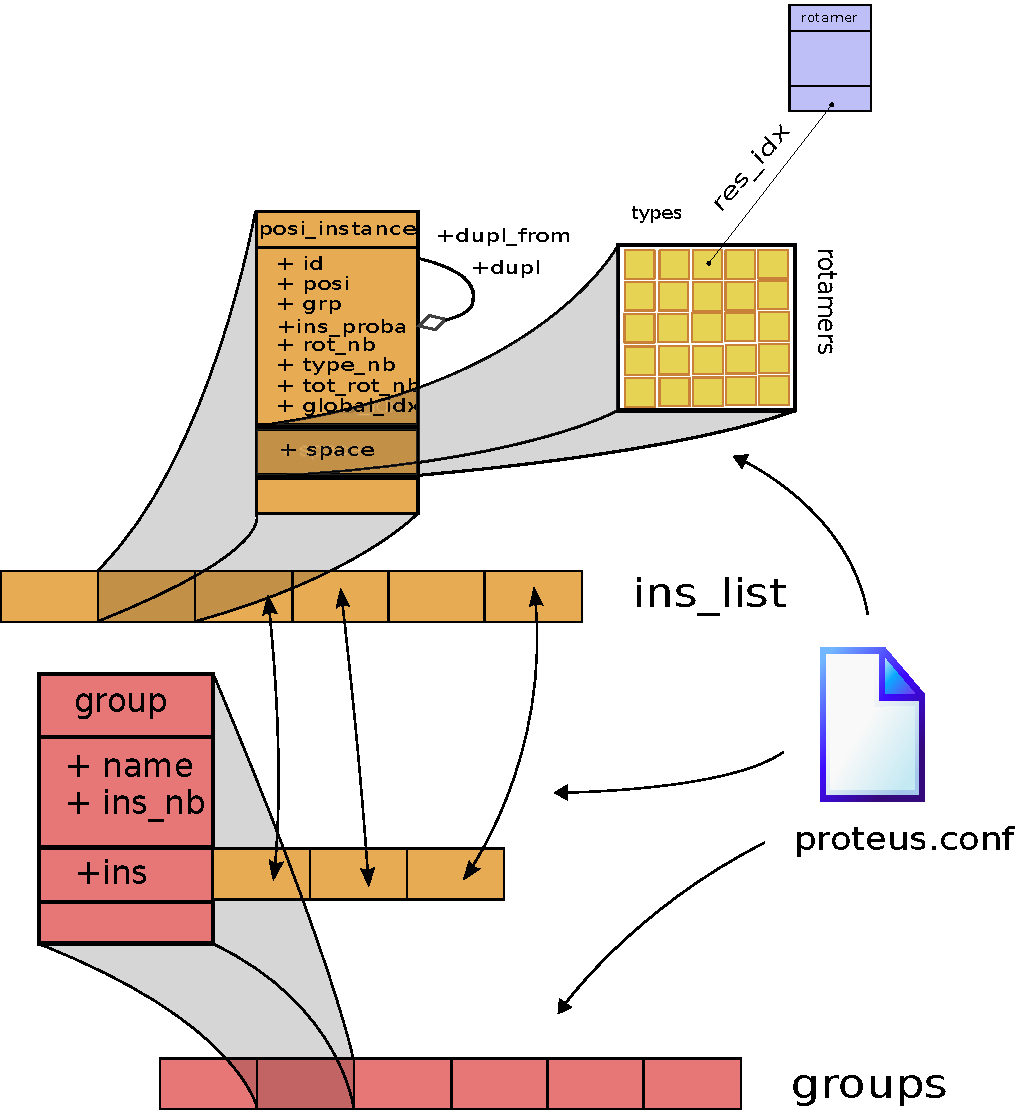
\includegraphics[width=16cm]{figure/structures_modele_logique.pdf} 
     \end{tabular}
     
     \caption{Les principales structures \og logiques\fg  dans proteus}
\label{fig:structLog}
   \end{figure}
   
Le dernier ensemble de structures de données contient les éléments régulièrement modifiés au cours de l'exploration.
Il y a un tableau  \verb!grp_ener! contenant les énergies de groupes ou interactions entre groupes utilisées dans la fonction de score. Il représente la partie utile de la matrice de la figure \ref{fig:groupmatrix}. La structure \verb!conformation! contient la séquence-conformation courante. Une liste de structures \verb!ins_modif! représente les modifications à effectuer sur la conformation courante, figure \ref{fig:structDyna}. Ceci permet la mise à jour des différentes énergies au cours de la trajectoire.   

   \begin{figure}[!htbp]
%     \centering
     \begin{tabular}{c}
       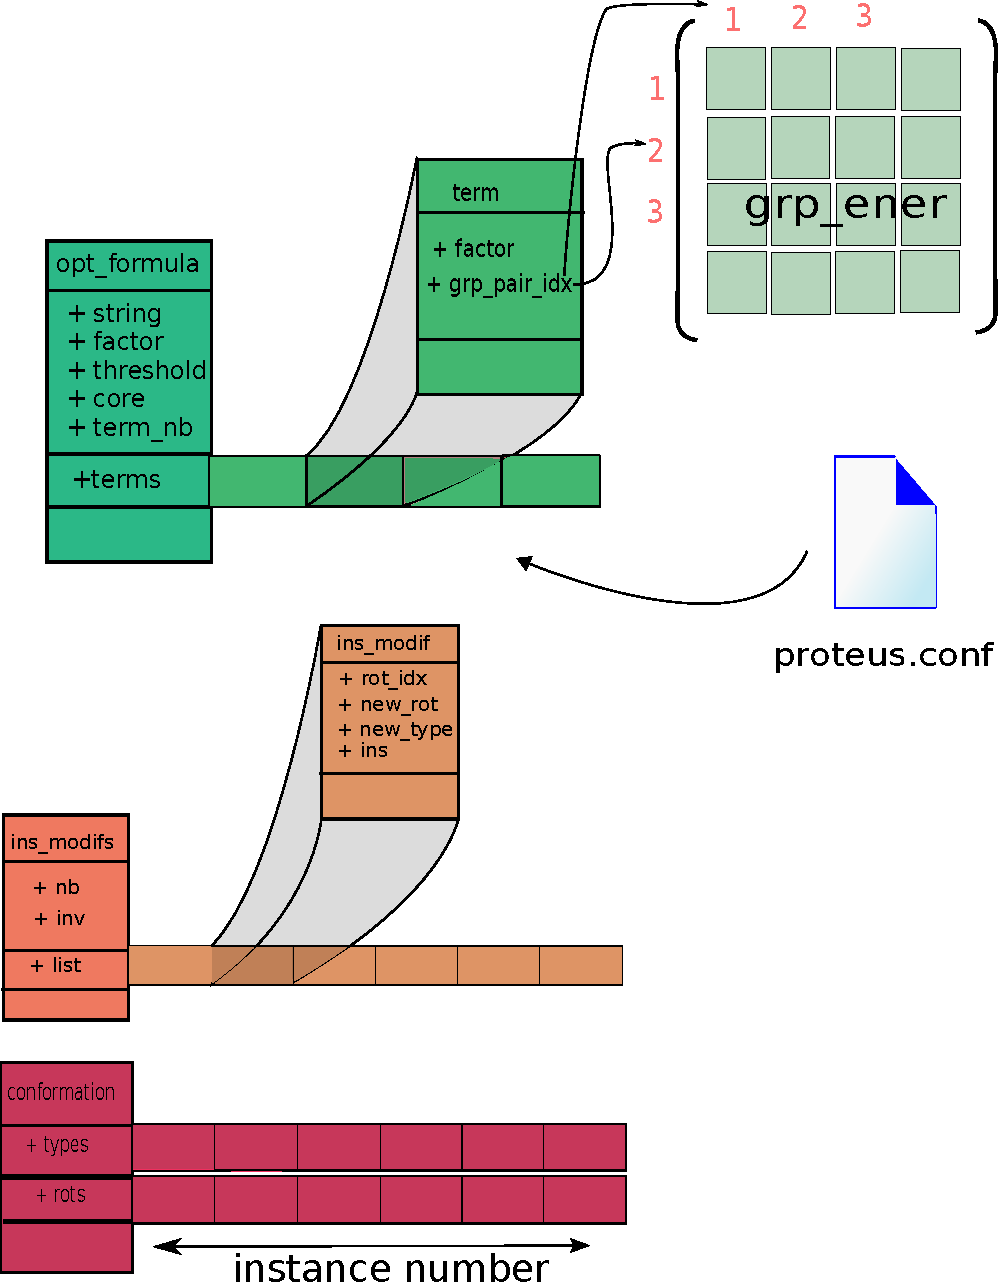
\includegraphics[width=16cm]{figure/structures_dynamiques.pdf} 
     \end{tabular}
     
     \caption{Les principales structures \og dynamiques\fg dans proteus}
\label{fig:structDyna}
   \end{figure}


%%% Local Variables:
%%% mode: latex
%%% TeX-master: "these"
%%% End:
